%   %==========================================================================
%   %  Section : 微分
%   %==========================================================================
        %==================================================================
        %  SubSection
        %==================================================================
            \subsection{変化の割合}
            一変数関数 $y=f(x)$ の変化の割合 $a$ を考える.関数 $f(x)$ が一次関数
            ($y=ax+b$)であるならば,$a$ は簡単に求めることができて,
            \begin{equation*}
                a=\frac{y\mbox{の増加量}}{x\mbox{の増加量}}
            \end{equation*}
            である
                \footnote{
                    変化の割合は,$x$ を変数としてもつ1次関数 $y$ が,$x$ が1だけ変化したときに
                    との程度変化するかを表すものである.この値により,$y$ の増加の仕方が
                    数量的にわかることになる.
                }.
            というか,これが変化の割合の定義である.一次関数上の異なる2点を任意にとっ
            て,その2点の座標をそれぞれ ($x_{1}\,,y_{1}$),($x_{2}\,,y_{2}$) とおく.
            ただし,$x_{1} < x_{2}$ とする.このとき変化の割合 $a$ は,
                \begin{equation*}
                    a = \frac{y_{2} - y_{1}}{x_{2} - x_{1}}
                \end{equation*}
            と計算すればよい.

        %==================================================================
        %  SubSection
        %==================================================================
            \subsection{「変化の割合」を拡張する}
            では,関数が2次関数や,三次関数,もっと複雑な $\sin x$ などのときの,変
            化の割合はどのようになるだろうか.一次関数の場合は,変化の割合は一定で
            あったが,2次関数やその他の一般の関数では,グラフの形からも想像できるよ
            うに,変化の割合は一定ではない.つまり,変化の割合は,グラフの各点でいろ
            んな値をとる.しかし,変化の割合がデタラメに決まっているわけではない.そ
            れはある決まった式によって書き表され,各点における変化の割合を計算す
            ることができる.

            例えば,2次関数 $y=x^{2}$ を考えてみよう.変化の割合は関数の2点の
            間で決定できるので,適当に関数上の点を2点とって,それを $x_{1}$,$x_{2}$ と
            しよう.ただし,$x_{1}<x_{2}$ であるとする.このとき,変化の割合は
            \begin{equation*}
                a = \frac{{x_{2}}^{2}-{x_{1}}^{2}}{x_{2}-x_{1}}
            \end{equation*}
            と計算される.しかし,$x_{1}$ と $x_{2}$ の間隔が大きいと,この変化の割
            合は図からわかるように,正確ではない.
                        \begin{figure}[hbt]
                            \begin{center}
                                \includegraphicslarge{2jikannsuu.pdf}
                                \caption{2次関数}
                                \label{fig:2jikannsuu}
                            \end{center}
                        \end{figure}

            そこで,2点 $x_{1}$,$x_{2}$ の間の距離を小さくしていくことで,近似的に,
            関数の傾き近づけていくことを考える.2点の間の大きさを $\Delta x$ とおいたとき,
            この $\Delta x$ を0に近づけていけばよい.この $\Delta x$ を用いることで,
            $x_{2}$ は
            \begin{equation*}
                x_{2}=x_{1}+\Delta x
            \end{equation*}
            と書ける.これを,さっきの2次関数の変化の割合の式に代入すると,
            \begin{equation*}
                a = \frac{{x_{2}}^{2}-{x_{1}}^{2}}{x_{2}-x_{1}}
                = \frac{({x_{1}+\Delta x})^{2}-{x_{1}}^{2}}{(x_{1}+\Delta x)-x_{1}}
                = \frac{2x_{1}\Delta x +\Delta x^{2}}{\Delta x}
                = 2x_{1} + \Delta x.
            \end{equation*}
            ここで,$\Delta x$ をできる限り0に近づけて,第一項の $2x_{1}$ に比べて無視できる
            程度にしたとき
                \footnote{
                    より詳細は,\textbf{極限} という概念を用いて考えないといけないのだが,
                    ここでは簡単のために,極限の概念を軽視した.
                },
            \begin{equation*}
                a = 2x_{1}
            \end{equation*}
            となる.ところで,この式は点 $x_{1}$ の部分だけに適用できるものだが,
            $x_{1}$ が任意に選べることから,
            \begin{equation*}
                a = 2x
            \end{equation*}
            であることがわかる.
            これが2次関数の変化の割合になる.一次関数との違いは,変化の割合が $x$ の関数
            になっていることだろう.これによって,2次関数の,全ての点における変化の割合
            を求めることができる.例えば,$x=1$ の部分における2次関数の傾きは,
            $a=2 \times 1 = 2$ と計算されるし,$x = 50$ の場合は,
            $a=2 \times 50 = 100$ である.少し計算は複雑になるが,
            一般の2次関数 $y=ax^{2}+bx+c$ の変化の割合は,これと同様な方法で求めることができて,
            \begin{equation*}
                a = 2ax + b
            \end{equation*}
            である.また,これと同様な方法で,$y=x^{3}$の変化の割合を求めることができる.
            三次関数の変化の割合の式は,$a = 3x^{2}$ となる.

        %==================================================================
        %  SubSection
        %==================================================================
            \subsection{導関数の定義(「微分する」ということ)}
            この計算方法を一般化してみよう.しかし,難しくなることを恐れて,関数は
            一変数関数 $y=f(x)$ としよう.点 $x$ における,$f(x)$ の変化の割合を求める.
            変化の割合を求めるには,関数上の2点($x$ ともう一点)が必要手である.しかし,この2点の間隔が
            大きすぎると,先ほどの例のように,正確に求めることができなくなる.そこで,
            もう1つの点を $x$ の近くにとるようにしたい.この点を,$x+\Delta x$ としよう.
            $\Delta x$ は非常に小さいけれども,0ではない数とする.
                \begin{figure}[hbt]
                    \begin{center}
                        \includegraphicslarge{bibunn1.pdf}
                        \caption{$\Delta x$ を0に近づけることで,関数の傾きの正確さが増す}
                        \label{fig:bibunn1}
                    \end{center}
                \end{figure}

            これらを,変化の割合の式に
            代入すると,
            \begin{equation*}
                a=\frac{y\mbox{の増加量}}{x\mbox{の増加量}}
                =\frac{f(x+\Delta x)-f(x)}{(x+\Delta x)-x}
                =\frac{f(x+\Delta x)-f(x)}{\Delta x}.
            \end{equation*}
            ここで,$\Delta x$ を0に近づけることを表現するため,
            $\displaystyle \lim_{\Delta x\rightarrow 0}$ という記号を導入する.
            \begin{equation*}
                a=\lim_{\Delta x\rightarrow 0}\frac{f(x+\Delta x)-f(x)}{\Delta x}.
            \end{equation*}
            関数 $f(x)$ の変化の割合を求める式を \textbf{導関数} という.また,
            そのような行為のことを,\textbf{微分する} という.
            $f(x)$ の導関数を表す記号として,
            \begin{align}
                f'(x)\,,\;\frac{\df f(x)}{\df x}\,,\;\frac{\df f}{\df x}(x)
            \end{align}
            等が用いられる.このノートでは,$f'(x)$ や $\df f(x)/\df x$ という記号を
            用いる.関数 $f(x)$ を微分するには\\

            \begin{itembox}[l]{導関数の定義(「微分する」という行為)}
            \begin{align}
                f'(x)=\frac{\df f(x)}{\df x}:=\lim_{\Delta x\rightarrow 0}\frac{f(x+\Delta x)-f(x)}{\Delta x}.
            \end{align}
            \end{itembox}\\

            以上の説明はあまりにも感覚的過ぎるので,
            微分積分の教科書で学習してもらいたい.ここでは,あくまでも
            イメージを優先した.また,以降の項目において,説明が楽になるようにと
            考えたためでもある.まあ,物理学に触れてみる程度ならば,この程度の
            説明で事足りると思う.

        %==================================================================
        %  SubSection
        %==================================================================
            \subsection{微分($\df y$の形式的定義)}
            \begin{mycomment}
                「微分」について説明よう.ちなみに,上では「微分する」
                という行為を定義した.それは,導関数の定義でもあった.
                    \begin{align*}
                        f'(x) = \frac{\df f(x)}{\df x}
                              = \lim_{\Delta x\rightarrow 0}\frac{f(x+\Delta x)-f(x)}{\Delta x}.
                    \end{align*}
                しかし,これと「微分」は異なる概念である.上の導関数の定義式の,
                $\df x$,$\df y$ には,定義上,なんの意味も与えられていない.
                $\df y/ \df x$ と書かれて,初めて導関数を意味するのであって,
                単独では意味を成さないのである.たしかに,$\df x$ は $\Delta x$ の
                0の極限として($\df y$ も同様),イメージされるかもしれないが,
                あくまでイメージであり,意味付けはされていない.そこで,ここで,
                新たに「微分」という概念を定義することで,$\df x$,$\df y$ に意味
                をもたせよう.そうすることで,$\df x$,$\df y$ を,あたかも変数で
                あるかのようにみなすことができ,式変形が容易に行えるようになる.
            \end{mycomment}

            導関数の公式の,極限 $\Delta x\rightarrow 0$ を\textbf{とる前の}
            式は,
                \begin{equation*}
                    \frac{\Delta y}{\Delta x}
                    = \frac{f(x+\Delta x)-f(x)}{\Delta x}.
                \end{equation*}
            である.これを,次のように変形させよう.
            \begin{equation*}
                \Delta y = f(x+\Delta x)-f(x).
            \end{equation*}
            両辺を $\Delta x(\neq 0)$ 倍しただけである.
            この式で,$\Delta x$ はとても小さいが,0の極限値を取っていないので,
            普通の実数であるから,このような除算が可能である.

            ここで,もう一度,今度は導関数の定義式より.
                \begin{align*}
                    f'(x) = \frac{\Delta y}{\Delta x}+o(\Delta x).
                \end{align*}
            ここに,今さっき求めた $\Delta y = f(x+\Delta x)-f(x)$ を考慮した.
            そして,さらに,極限 $\Delta x\rightarrow 0$ を取ることを省いた.
            そのため,$o(\Delta x)$ という余分な項が付いている.これは,極限を
            とる操作を省いたために生じた,誤差を表現したものである.
            両辺を $\Delta x$ 倍しよう.
                \begin{equation*}
                    f'(x) \Delta x = \Delta y + o(\Delta x)\Delta x.
                \end{equation*}

            ここで,\textbf{微分}  $\df y= \df f(x)$ を次式で定義する.
                \begin{align}
                    \df y = \df f(x) := f'(x)\Delta x.
                \end{align}

            微分 $\df y$ を使うと,
                \begin{align}
                    \df y = \Delta y + o(\Delta x)\Delta x.
                \end{align}
            つまり,この微分 $\df y$ は,
            「$x$ が $\Delta x$ だけ変化したときの $y$ の増分」を表す.

            上式の $o(\Delta x)\Delta x$ は,$\Delta x \rightarrow 0$ としたときに
            0に近づく量であるので,この極限を再び考慮すると,
                \begin{align}
                    \df y = \Delta y \,,\quad (\Delta x \rightarrow 0).
                \end{align}
            この式から,$\Delta x \rightarrow 0$ の極限をとると,微分 $\df y$ は,
            $y$ の変化分 $\Delta y$ と同一視できることがわかる.

            図を用いたイメージでも説明できるが,そのためには,接線の方程式について
            の知識があるとよい.そこで,次節で接線の方程式を復習したあとで,$\df y$ の
            図形的イメージを紹介しよう.\\

            \begin{itembox}[l]{微分の定義}
            \textbf{微分}  $\df y= \df f(x)$ を次式で定義する.
                    \begin{align}
                        \df y = \df f(x) := f'(x)\Delta x.
                    \end{align}
            である.
            \end{itembox}

            \begin{memo}{独立変数 $x$ の微分}
                $x$ は関数 $f(x)$ の独立変数としているが,この $x$ 自身の
                微分 $\df x$ はどう表されるだろうか.ここで計算しておこう.
                定義式は $y$ についての微分 $\df y$ について記述された式
                であるが,$y$ は任意であるので,当然,$y=f(x)=x$ の場合も考えられる.
                つまり,
                    \begin{align}
                        \df x = \df f(x) = f'(x)\Delta x = 1\,\Delta x = \Delta x.
                    \end{align}
                要するに,独立変数 $x$ の微分 $\df x$ は,それ自身の変化分 $\Delta x$ に
                同じであると言える.
            \end{memo}

            \begin{memo}{導関数の式}
                上の計算から,
                微分の定義式 $\df y:=f'(x)\Delta x$ の $\Delta x$ は $\df x$ に置き換える
                ことができて,
                    \begin{equation*}
                        \df y=f'(x)\df x
                    \end{equation*}
                上式を次のように変形させれば,導関数の定義と同じ式を得る.
                    \begin{align}
                        \frac{\df y}{\df x}=f'(x).
                    \end{align}
            \end{memo}

        %==================================================================
        %  SubSection
        %==================================================================
            \subsection{(関数 $f(x)$ の)接線の方程式}
            関数 $f(x)$ の,点 $\alpha$ における,接線の方程式を求める.

            接線の方程式とは,直線の方程式であり,$y=ax+b$ と書かれる.
            一般の関数 $f(x)$ に対して,
            導関数 $f'(x)$ を求めることにより,
            関数 $f(x)$ の各点における変化の割合が求まる.
            ということは,$a=f'(\alpha)$ として,$y=f'(\alpha)x+b$ と書き表せる.
            関数 $f(x)$ は,$x=\alpha$ のとき,点$(\,\alpha,\,f(\alpha)\,)$ を通る.
            つまり,方程式 $y=f'(\alpha)x+b$ に $y=f(\alpha)$,$x=\alpha$ を代入し,
                \begin{equation*}
                    f(\alpha) = f'(\alpha)\alpha + b
                \end{equation*}
            が成立しているはずである.これと,元の式
                \begin{equation*}
                    y=f'(\alpha)x+b
                \end{equation*}
            の両辺を引くことで,
                \begin{align*}
                    y - f(\alpha) &=   \left( f'(\alpha)x      + b \right)
                                      - \left( f'(\alpha)\alpha + b \right) \\
                                  &= f'(\alpha) \left( x-\alpha \right)
                \end{align*}
            と計算される.これが接線の方程式である.\\

            \begin{itembox}[l]{接線の方程式}
            関数 $f(x)$ の,$x=\alpha$ における,接線の方程式は,
            \begin{align}
                y - f(\alpha)=f'(\alpha) \left( x-\alpha \right)
            \end{align}
            である.
            \end{itembox}

        %==================================================================
        %  SubSection
        %==================================================================
            \subsection{$\df y$ の図形的イメージ}
                このように微分を定義することで,$\df y$ に次のような意味が
                与えられる.
                \begin{figure}[hbt]
                    \begin{center}
                        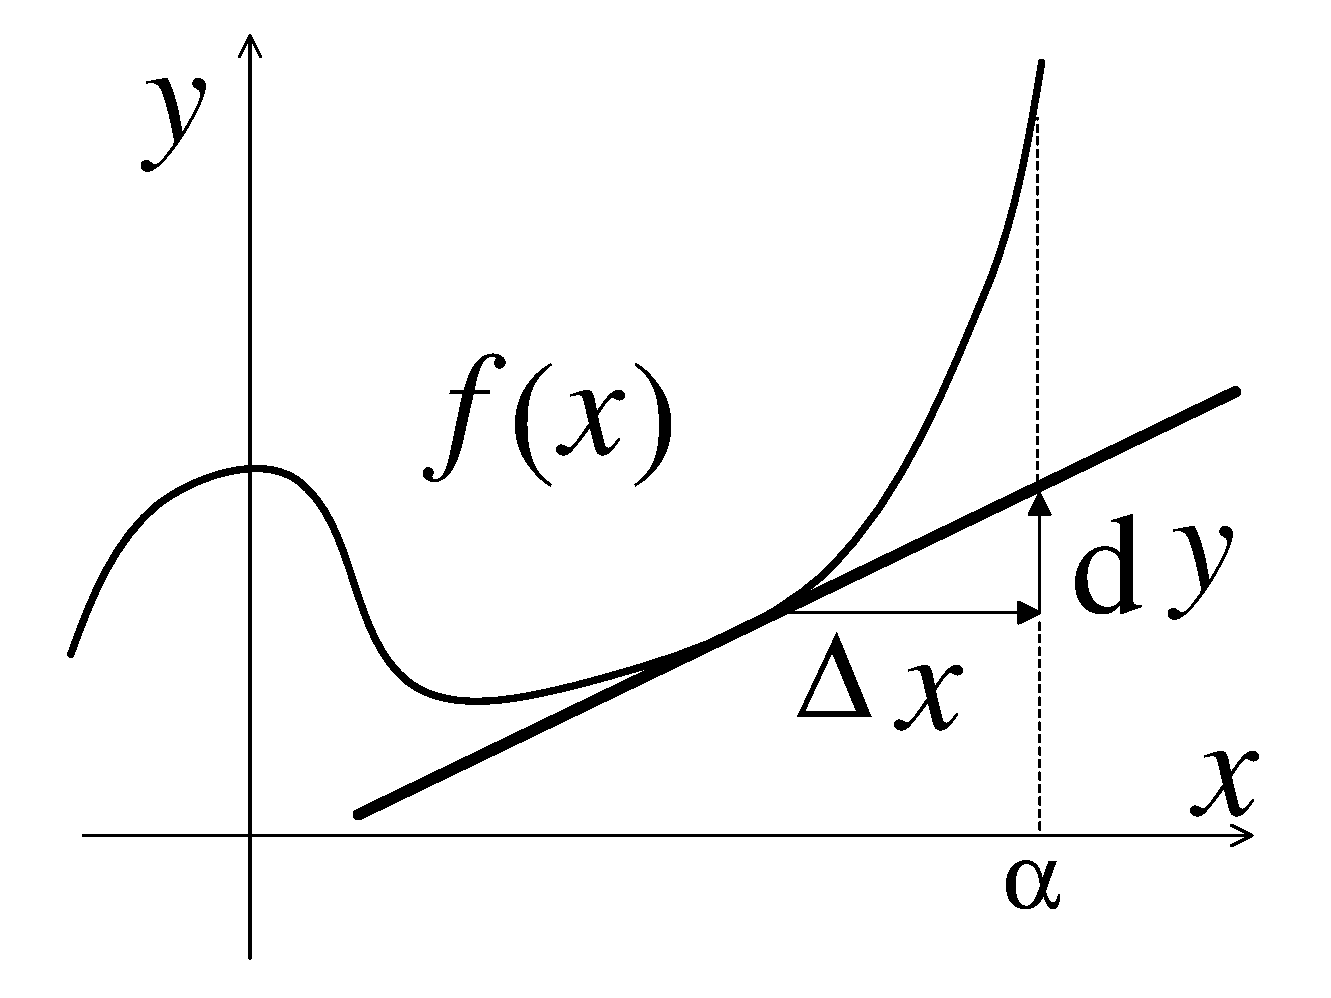
\includegraphics[keepaspectratio, width=6cm,height=2.4cm,clip]{bibunnno_Teigi00.pdf}
                        \caption{微分の定義}
                        \label{fig:bibunnno_Teigi00}
                    \end{center}
                \end{figure}

        %==================================================================
        %  SubSection
        %==================================================================
            \subsection{1次関数 $f(x)=ax+b$ の増加量}
                一次関数の増加量を,微分を使って表してみる.仰々しいかもしれないが,
                後でこの考え方を発展させるために,基礎的なところから考えていきたい.
                \begin{figure}[hbt]
                    \begin{center}
                        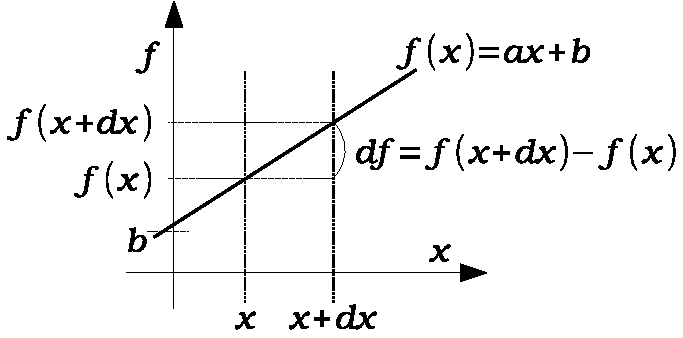
\includegraphics[keepaspectratio, width=6cm,height=2.85cm,clip]{ichi_hensu_kansu_zokaryo2.pdf}
                        \caption{1次関数数関数 $f(x)=ax+b$ の増加量}
                        \label{fig:ichi_hensu_kansu_zokaryo2}
                    \end{center}
                \end{figure}

                一次関数はグラフで表現すると直線であり,
                方程式は $f(x)=ax+b$ である.$a$ は傾きで,$b$ は $y$ 軸との交点である
                        \footnote{
                                $b$ は切片ともよばれる.
                        }.
                                点 $x$ のところでは,
                                        \begin{equation*}
                                                f(x) = ax + b.
                                        \end{equation*}
                                点 $x$ から微小距離 $\df x$ だけ離れたところでは($x+\df x$),
                                        \begin{equation*}
                                                f(x+\df x)=a(x+\df x)+b.
                                        \end{equation*}
                                よって, $x$ が $\df x$ だけ増えた時の $f(x)$ の増加量を $\df f$ として
                                        \footnote{
                                                より細かく表現すると,$\df f := \df f(x)$ である.
                                        },
                                        \begin{align*}
                                                \df f &= f(x+\df x) - f(x) \\
                                                      &= \{a(x+\df x)+b\} - \{ax + b\} \\
                                                      &= (ax + a\df x + b) - (ax + b) \\
                                                      &= a \df x.
                                        \end{align*}

                                一次関数の増加量は傾き $a$ と 微少変化 $\df x$ の積で表せることがわかった.

        %==================================================================
        %  SubSection
        %==================================================================
            \subsection{1変数関数 $f(x)$ の増加量}
                1変数関数 $f(x)$ において,$x$ の微小変化分 $\df x$ に対する $f(x)$ の
                増加量を計算したいことがある.これは,局所的に一次関数近似することで,
                一次関数の時と同じように考えることができる.
                \begin{figure}[hbt]
                    \begin{center}
                        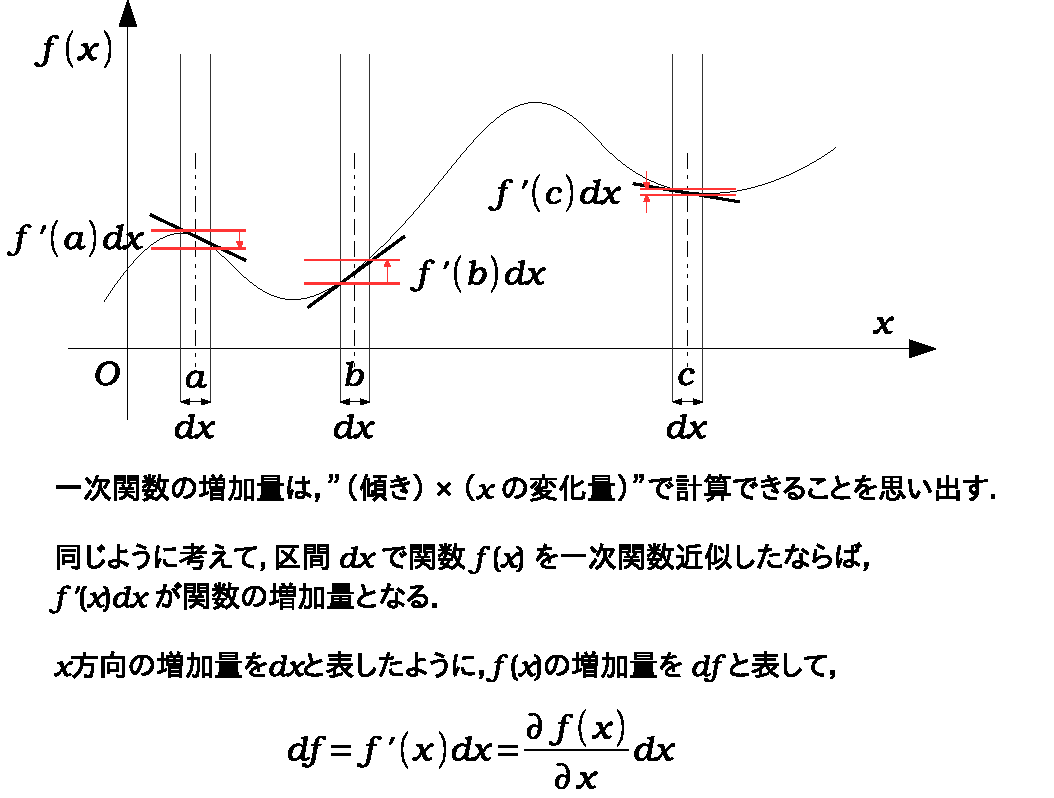
\includegraphics[keepaspectratio, width=7cm,height=6.7cm,clip]{ichi_hensu_kansu_zokaryo1.pdf}
                        \caption{1変数関数 $f(x)$ の増加量}
                        \label{fig:ichi_hensu_kansu_zokaryo1}
                    \end{center}
                \end{figure}

                                一次関数では,微小変化 $\df x$ に対する関数$f$の増加量は,
                                $\df f= a\df x$ と書けるのであった.
                                これを任意の一変数関数に拡張する場合,各$x$ で傾きが異なるが,$a=f'(x)$ と書けることを考慮すると,
                                        \begin{align}
                                                \df f = f'(x) \df x
                                        \end{align}
                                となる.これが1変数関数 $f(x)$ の増加量である.これはまさに,
                                前に説明した \textbf{微分} にほかならない.微分とは一変数関数の微小増加量のことをいうのである.

        %==================================================================
        %  SubSection
        %==================================================================
            \subsection{偏微分}
                次は2変数関数の微分だ.
                1変数関数のグラフは線であり,$x$方向の1方向のみを考えればよかった.
                これに対して,2変数の場合は面になるので,$x$方向と$y$方向の2方向を
                考える必要がある.

                $x$方向の微分をする場合は,$y$方向を固定して微分する.
                式で書くと,
                        \begin{equation*}
                                \frac{\rd f(x,\,y)}{\rd x}
                                := \lim_{\Delta x \to 0} \frac{f(x+\Delta x,\,y)-f(x,\,y)}{\Delta x}.
                        \end{equation*}
                $y$方向の微分をする場合は,$x$方向を固定して微分する.
                式で書くと,
                        \begin{equation*}
                                \frac{\rd f(x,\,y)}{\rd y}
                                := \lim_{\Delta y \to 0} \frac{f(x,\,y+\Delta y)-f(x,\,y)}{\Delta y}.
                        \end{equation*}
                このような微分を1変数の微分と区別するために
                        \footnote{
                                言い換えれば,多変数関数の微分であることを\textbf{強調}するために.
                        },
                \textbf{偏微分} という.

                偏微分の視点で,改めて,1変数の微分を見ると,$y=0$ 固定の微分であったと解釈できる.

        %==================================================================
        %  SubSection
        %==================================================================
            \subsection{全微分}
                偏微分の場合,微分するときに片方を固定してしまうので,$x$ と $y$ を"同時に"変化させた場合
                の関数の増加量がわからない.幸運なことに,$x$ と $y$ を"同時に"変化させた場合の増加量は,
                それぞれ独立であり,
                従って,「$x$ だけを変化させた場合の増加量」と「$y$ だけを変化させた場合の増加量」を
                たすだけで良い.
                \begin{figure}[hbt]
                    \begin{center}
                        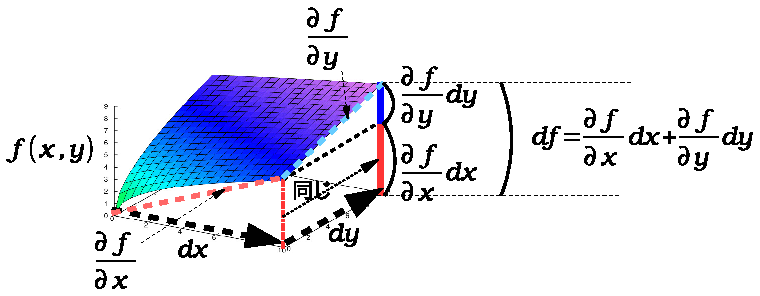
\includegraphics[keepaspectratio, width=7cm,height=4.096cm,clip]{gradient_sample_figure_0001.pdf}
                        \caption{全微分のイメージ}
                        \label{fig:gradient_sample_figure_0001}
                    \end{center}
                \end{figure}

                                $x$ 方向だけ変化させた場合の増加量とは,$x$ 方向についての微分であり,
                                        \begin{equation*}
                                                \frac{\rd f(x,\,y)}{\rd x} \df x
                                        \end{equation*}
                            である.また,$y$ 方向だけ変化させた場合の増加量とは,$y$ 方向についての微分であり,
                                        \begin{equation*}
                                                \frac{\rd f(x,\,y)}{\rd y} \df y
                                        \end{equation*}
                            と書ける.よって,$\df f:=\df f(x,\,y)$ は
                                \begin{align}
                                        \df f = \frac{\rd f(x,\,y)}{\rd x} \df x + \frac{\rd f(x,\,y)}{\rd y} \df y
                                \end{align}
                            と計算することができる.

                            このような2変数関数の微分のことを \textbf{全微分} という
                                \footnote{
                                                1変数関数の微小増加量が微分であることを先に確認した.
                                2変数関数の場合は方向が2つあるので,増加量を計算するには全方向の微分を
                                足し合わせるのであった.これを強調し,2変数関数の微分のことを \textbf{全微分} という.
                                2変数以上の関数の微分は全て,全微分と言われる.
                                }.
